% ======================================================================
%  Chapter 15 — Weyl Points of Maxwell Bands  (EXPANDED)
% ======================================================================

\section{From two dimensions to three}
\label{sec:ch15-2d-to-3d}

In two dimensions, Dirac points are degeneracies that can be gapped by
time-reversal or inversion breaking, producing bands with nonzero Chern
numbers.  In \emph{three} dimensions, a qualitatively new type of
topological degeneracy appears: the \emph{Weyl point}, a point in 3D
momentum space where two bands touch linearly.  Unlike 2D Dirac points,
Weyl points are \emph{topologically robust}: they cannot be gapped by
any perturbation, only moved in $\kvec$-space or annihilated in pairs.

Weyl points are Berry-curvature monopoles---point sources or sinks of
Berry flux in 3D momentum space \cite{ozawa2018topological}.  Their existence has profound
consequences for surface physics: the surface Brillouin zone contains
open Fermi arcs connecting the projections of Weyl points of opposite
chirality
\cite{hsieh2008topological,armitage2018weyl}.

\section{The three-dimensional Maxwell eigenproblem}
\label{sec:ch15-3d-maxwell}

\subsection{Extension to three dimensions}
\label{sec:ch15-extension}

The Maxwell eigenvalue equation $\Maxop(\kvec)\mathbf{u}=\omega\Mmat
\mathbf{u}$ extends directly to three dimensions.  The Bloch wavevector
$\kvec=(k_x,k_y,k_z)$ lives in a 3D Brillouin zone, which for a cubic
lattice is a cube $[-\pi/a,\pi/a]^3$ (with opposite faces identified,
forming a 3-torus $T^3$).  The cell-periodic eigenmodes
$\mathbf{u}_{n\kvec}(\rvec)$ and eigenfrequencies $\omega_{n\kvec}$
depend on all three components of $\kvec$.

\subsection{Berry curvature as a vector field}
\label{sec:ch15-berry-vector}

In 3D, the Berry curvature is naturally a vector field in
$\kvec$-space:
\begin{equation}\label{eq:ch15-berry-3d}
  \boldsymbol{\Omega}_n(\kvec)
  = \nabla_\kvec\times\Aberryvec_n(\kvec)\,,
\end{equation}
where $\Aberryvec_n(\kvec)=\ii\langle\mathbf{u}_{n\kvec}|\Mgmat
|\nabla_\kvec\mathbf{u}_{n\kvec}\rangle$ is the Berry connection
vector.  The Berry curvature satisfies
$\nabla_\kvec\cdot\boldsymbol{\Omega}_n=0$ everywhere except at band
degeneracies, where it has point sources or sinks (monopoles).

\subsection{Chern numbers on 2D slices}
\label{sec:ch15-slices}

For any 2D slice of the 3D Brillouin zone at fixed $k_z$, we can
compute the Chern number:
\begin{equation}\label{eq:ch15-slice-chern}
  \Chern_n(k_z) = \frac{1}{2\pi}\int_{k_z=\mathrm{const}}
  \Omega_{n,z}\,\dd k_x\,\dd k_y\,
\end{equation}
The displayed formula above follows the convention and normalisation used in \cite{zhao2020first}.
This is the ``Chern number of the $k_z$-slice.''  It is an integer that
can only change when the slice passes through a Weyl point (where the
band gap closes).  The change in $\Chern_n(k_z)$ across a Weyl point
equals the chirality of that Weyl point.

\section{Weyl points as Berry monopoles}
\label{sec:ch15-monopoles}

\subsection{The 3D Weyl Hamiltonian}
\label{sec:ch15-weyl-hamiltonian}

Near a Weyl point at $\kvec=\kvec_W$ in a 3D band structure, the
effective $2\times 2$ Hamiltonian takes the form
\begin{equation}\label{eq:ch15-weyl-hamiltonian}
  \boxed{%
  H_W(\delta\kvec) = \sum_{a=x,y,z} v_a\,\delta k_a\,\sigma_a\,,}
\end{equation}
where $\delta\kvec=\kvec-\kvec_W$ and $v_a$ are the anisotropic
velocities.  This is the 3D generalisation of the 2D massless Dirac
equation, but with all three Pauli matrices present.

The eigenvalues are
\begin{equation}\label{eq:ch15-weyl-dispersion}
  E_\pm(\delta\kvec) = \pm\sqrt{v_x^2\delta k_x^2
  +v_y^2\delta k_y^2+v_z^2\delta k_z^2}\,,
\end{equation}
giving a point-like band touching with linear (conical) dispersion in
all three momentum directions.  The constant-energy surfaces are
ellipsoids centred at $\kvec_W$.

\subsection{Derivation of the Berry curvature monopole}
\label{sec:ch15-monopole-derivation}

For the isotropic case $v_x=v_y=v_z\equiv v$, the Weyl Hamiltonian
reduces to $H=v\,\delta\kvec\cdot\boldsymbol{\sigma}$.  Using the
general formula for a two-band Hamiltonian $H=\mathbf{d}\cdot
\boldsymbol{\sigma}$:
\begin{equation}\label{eq:ch15-general-berry}
  \Omega_{n,a}
  = -\frac{\chi}{2}\,\epsilon_{abc}\,
  \hat{d}_b\Bigl(\pderiv{\hat{d}_c}{\delta k_d}\times
  \pderiv{\hat{d}_d}{\delta k_e}\Bigr)_{de}
  \quad\Longrightarrow\quad
  \boldsymbol{\Omega}_-
  = -\frac{\chi}{2}\,\frac{\delta\kvec}{|\delta\kvec|^3}\,,
\end{equation}
where $\chi=\sgn(\det[v_{ab}])=\pm 1$ is the chirality.

More explicitly, for $\mathbf{d}=v\delta\kvec$ and
$\hat{\mathbf{d}}=\delta\kvec/|\delta\kvec|$:
\begin{align}
  \Omega_{-,x} &= -\frac{\chi}{2}\,
    \frac{\delta k_x}{(\delta k_x^2+\delta k_y^2+\delta k_z^2)^{3/2}}\,,\\
  \Omega_{-,y} &= -\frac{\chi}{2}\,
    \frac{\delta k_y}{(\delta k_x^2+\delta k_y^2+\delta k_z^2)^{3/2}}\,,\\
  \Omega_{-,z} &= -\frac{\chi}{2}\,
    \frac{\delta k_z}{(\delta k_x^2+\delta k_y^2+\delta k_z^2)^{3/2}}\,.
\end{align}
This is the field of a magnetic monopole in momentum space, with charge
$-\chi$.  It diverges at $\delta\kvec=\mathbf{0}$ (the Weyl point)
and falls off as $1/|\delta\kvec|^2$.

\subsection{Topological charge and flux quantisation}
\label{sec:ch15-charge}

The flux of Berry curvature through any closed surface $S$ enclosing
the Weyl point is quantised:
\begin{equation}\label{eq:ch15-monopole-flux}
  \boxed{%
  \frac{1}{2\pi}\oint_S\boldsymbol{\Omega}_-\cdot\dd\mathbf{S}
  = -\chi = \mp 1\,.}
\end{equation}

\begin{proof}
For a sphere of radius $R$ centred at the Weyl point:
\begin{align}
  \frac{1}{2\pi}\oint_{S^2}\boldsymbol{\Omega}_-\cdot\dd\mathbf{S}
  &= \frac{1}{2\pi}\int_0^\pi\int_0^{2\pi}
  \Bigl(-\frac{\chi}{2R^2}\Bigr)R^2\sin\theta\,\dd\theta\,\dd\phi
  \notag\\
  &= -\frac{\chi}{2}\cdot\frac{1}{2\pi}\cdot 4\pi = -\chi\,.
\end{align}
\end{proof}

This is the 3D analog of the half-integer Berry flux at a 2D Dirac
point, but in 3D the flux is \emph{integer} for a single Weyl point
(because the enclosing surface is a sphere $S^2$, which is a
closed orientable 2-manifold).

\subsection{Topological robustness}
\label{sec:ch15-robustness}

A key difference from 2D Dirac points: a Weyl point in 3D \emph{cannot
be gapped by any local perturbation}.

\begin{proposition}
  No perturbation of the form $\delta H=\sum_a\delta d_a\sigma_a
  +\delta d_0\mathbf{I}$ can open a gap at a Weyl point.  It can only
  shift the Weyl point in $\kvec$-space.
\end{proposition}

\begin{proof}
  The perturbed Hamiltonian is
  $H'=\sum_a(v_a\delta k_a+\delta d_a)\sigma_a+\delta d_0\mathbf{I}$.
  The gap closes when $v_a\delta k_a+\delta d_a=0$ for all $a$, i.e.,
  at $\delta k_a=-\delta d_a/v_a$.  The Weyl point has moved to
  $\kvec_W'=\kvec_W-(\delta d_x/v_x,\delta d_y/v_y,\delta d_z/v_z)$,
  but it has not been removed.  A general $2\times 2$ Hermitian matrix
  has 4 parameters ($d_0,d_x,d_y,d_z$), of which 3 must vanish for
  a degeneracy; with 3 free parameters $(\delta k_x,\delta k_y,
  \delta k_z)$, this is generically satisfied at isolated points.
\end{proof}

To remove a Weyl point, it must be brought together with another Weyl
point of \emph{opposite} chirality, where they annihilate.  This is the
momentum-space analog of monopole-antimonopole annihilation in
electrostatics.

This annihilation process is illustrated schematically in
Figure~\ref{fig:ch15-weyl-annihilation}.  Panel~(a) shows two well-separated
Weyl nodes of opposite chirality (blue~$=-1$, red~$=+1$) along a
one-dimensional momentum cut, each carrying a linear band crossing.  As a
tuning parameter is varied, the nodes move toward each other in panel~(b).
At the critical point---panel~(c)---the two charges become coincident and the
dispersion along the merging direction changes from linear to quadratic,
reflecting the cancellation of the net Berry monopole charge.  Beyond the
critical point, a full gap opens as shown in panel~(d), with gap
$E_g$ set by the distance past the transition.  The entire sequence is the
momentum-space counterpart of monopole--antimonopole pair annihilation in
classical electrostatics.

\begin{figure}[t]
  \centering
  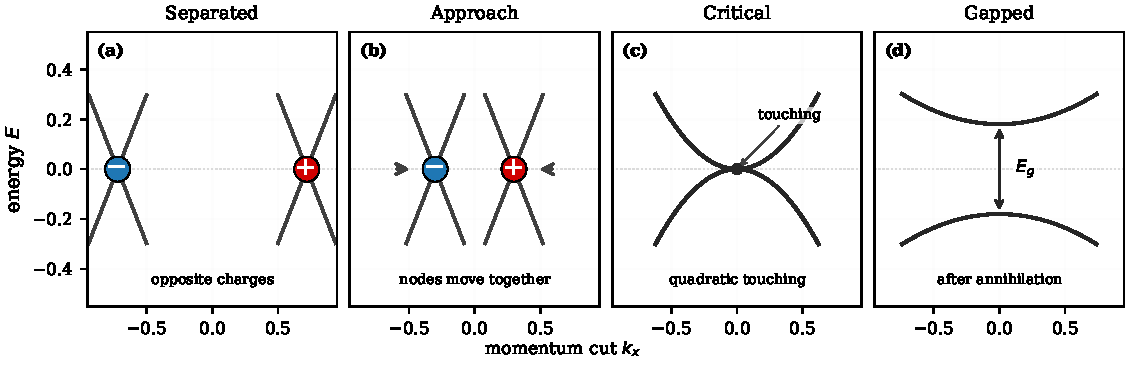
\includegraphics[width=\textwidth]{figures/fig_ch15_weyl_annihilation_step178.pdf}
  \caption{Weyl-point pair annihilation along a one-dimensional momentum cut
  $k_x$.
  (a)~Two separated Weyl nodes of opposite chirality: blue~$(\chi=-1)$,
  red~$(\chi=+1)$, each with a local linear crossing.
  (b)~The nodes approach as a lattice parameter is tuned.
  (c)~At the critical point the charges are coincident and the dispersion
  becomes quadratic along the merging direction; the net monopole charge
  vanishes.
  (d)~Beyond the transition a gap~$E_g$ opens; the resulting phase is
  topologically trivial in the Weyl sense.}
  \label{fig:ch15-weyl-annihilation}
\end{figure}

\subsection{The Nielsen--Ninomiya theorem in 3D}
\label{sec:ch15-nn}

In a compact 3D Brillouin zone (a torus $T^3$), the total monopole
charge must vanish:
\begin{equation}\label{eq:ch15-nn}
  \sum_i \chi_i = 0\,.
\end{equation}

\begin{proof}
The total Berry flux through the boundary of the Brillouin zone is
zero (because the torus has no boundary).  By Gauss's theorem, the
total enclosed charge vanishes.
\end{proof}

This means Weyl points always come in pairs of opposite chirality,
analogous to the pairing of 2D Dirac points (the
fermion-doubling theorem).

\section{Weyl points in photonic crystals}
\label{sec:ch15-photonic}

\subsection{Symmetry requirements}
\label{sec:ch15-symmetry}

A Weyl point requires the breaking of either time-reversal ($\Top$) or
inversion ($\Pop$) symmetry (or both).  The reason is as follows.

If both $\Top$ and $\Pop$ are present, the combined operation
$\Top\Pop$ is an anti-unitary symmetry that maps $\kvec$ to itself
(because $\Top:\kvec\to-\kvec$ and $\Pop:\kvec\to-\kvec$, so
$\Top\Pop:\kvec\to\kvec$).  Since $(\Top\Pop)^2=\Top^2\Pop^2=+1$ for
photons ($\Top^2=+1$, $\Pop^2=+1$), the anti-unitary constraint does
not force Kramers degeneracy.  However, the real-symmetric structure of
the combined eigenproblem typically enforces at least a twofold
degeneracy at every $\kvec$ point, making the minimal band touching a
four-fold Dirac point rather than a two-fold Weyl point.

Breaking either $\Top$ or $\Pop$ removes this constraint and allows
isolated two-fold Weyl points.

\subsection{Classification of photonic Weyl systems}
\label{sec:ch15-classification}

\begin{center}
\begin{tabular}{lccl}
  \toprule
  \textbf{Symmetry broken} & $\Top$ & $\Pop$ &
    \textbf{Example systems} \\
  \midrule
  Inversion only & yes & no &
    Chiral photonic crystals, asymmetric gyroid \\
  Time reversal only & no & yes &
    Gyromagnetic 3D crystals \\
  Both & no & no &
    General magneto-optic + chiral \\
  \bottomrule
\end{tabular}
\end{center}

The case of broken $\Pop$ with preserved $\Top$ is most common in
photonic experiments, because chiral 3D structures can be fabricated
by multi-layer lithography or 3D printing without requiring
magneto-optical materials \cite{lu2012weyl}.

\subsection{The double gyroid photonic crystal}
\label{sec:ch15-gyroid}

One of the first predicted photonic Weyl-point systems is based on the
gyroid minimal surface \cite{ozawa2018topological,liu2021observation}: a triply periodic surface that divides space
into two interpenetrating labyrinthine channels.

In the \emph{single} gyroid structure, the photonic crystal has
body-centred-cubic symmetry with both $\Top$ and $\Pop$.  The band
structure shows Dirac points (four-fold) at high-symmetry points.

In the \emph{double} gyroid, the two channels are filled with different
dielectric materials ($\varepsilon_1\neq\varepsilon_2$), breaking
$\Pop$ while preserving $\Top$.  Each four-fold Dirac point splits into
two Weyl points of opposite chirality, separated in $\kvec$-space by an
amount proportional to the asymmetry $|\varepsilon_1-\varepsilon_2|$.

The positions of the Weyl points in the Brillouin zone are constrained
by the remaining symmetries ($C_3$ rotations along the body diagonal),
which force the Weyl points to lie along high-symmetry lines.

\subsection{Stacked 2D photonic crystals}
\label{sec:ch15-stacked}

A simpler approach creates Weyl points by stacking identical 2D
photonic crystal layers with a controlled interlayer coupling.  If each
2D layer has Dirac points at $K$ and $K'$, the interlayer coupling
disperses these degeneracies along $k_z$, creating either:
\begin{itemize}
  \item A \emph{nodal line}: a continuous ring of degeneracies in
  $(k_x,k_y,k_z)$ space (when $\Top+\Pop$ is preserved)
\cite{kawabata2019symmetry}.
  \item \emph{Weyl points}: isolated degeneracies (when $\Pop$ or
  $\Top$ is broken by the stacking geometry or material choice).
\end{itemize}

The interlayer coupling strength $t_z$ controls the $k_z$-dispersion
and hence the separation of Weyl points.

\section{Surface states and Fermi arcs}
\label{sec:ch15-surface}

\subsection{The surface Brillouin zone}
\label{sec:ch15-surface-bz}

Consider a semi-infinite 3D photonic crystal with a surface perpendicular
to $\hat{x}$.  The surface states are labelled by the surface-parallel
wavevector $\kvec_\parallel=(k_y,k_z)$ and form a 2D band structure
$\omega_{\mathrm{surf}}(\kvec_\parallel)$~\cite{kane2005sub}.

\subsection{Derivation of Fermi arcs from slice Chern numbers}
\label{sec:ch15-arcs-derivation}

The existence of surface states can be understood through the
$k_z$-dependent Chern number $\Chern_n(k_z)$ defined in
\eqref{eq:ch15-slice-chern}.

Consider the 2D slice at a given $k_z$.  If $\Chern_n(k_z)\neq 0$,
the bulk-edge correspondence for 2D systems
(Theorem~\ref{thm:ch8-bec}) predicts $|\Chern_n(k_z)|$ chiral edge modes
at the surface.  These edge modes have a definite group velocity along
$k_y$ and appear at a specific frequency $\omega_{\mathrm{edge}}(k_y,k_z)$.

As $k_z$ sweeps between two Weyl points of opposite chirality at
$k_{z,1}$ and $k_{z,2}$, the Chern number changes from $+1$ to $0$
(or $0$ to $-1$, etc.).  In the region where $\Chern(k_z)=1$, there is
one surface mode; outside this region, there is none.  The surface mode
therefore exists only for $k_z\in(k_{z,1},k_{z,2})$, tracing an
\emph{open arc} in the surface Brillouin zone.

At a fixed frequency equal to the Weyl-point frequency, this arc is
called a \emph{Fermi arc} (by analogy with the electronic case).  The
Fermi arc connects the projections of the two Weyl points onto the
surface Brillouin zone.

\begin{remark}
  The Fermi arcs are \emph{open} curves, not closed loops.  This is
  topologically possible because the arcs terminate at the projected
  Weyl points, where the surface states merge into the bulk continuum.
  Open Fermi arcs have no analog in 2D topological systems, where edge
  modes always form closed dispersion curves crossing the bulk gap.
\end{remark}

Figure~\ref{fig:ch15-weyl-chern-slices} summarises this structure
schematically.

\begin{figure}[t]
  \centering
  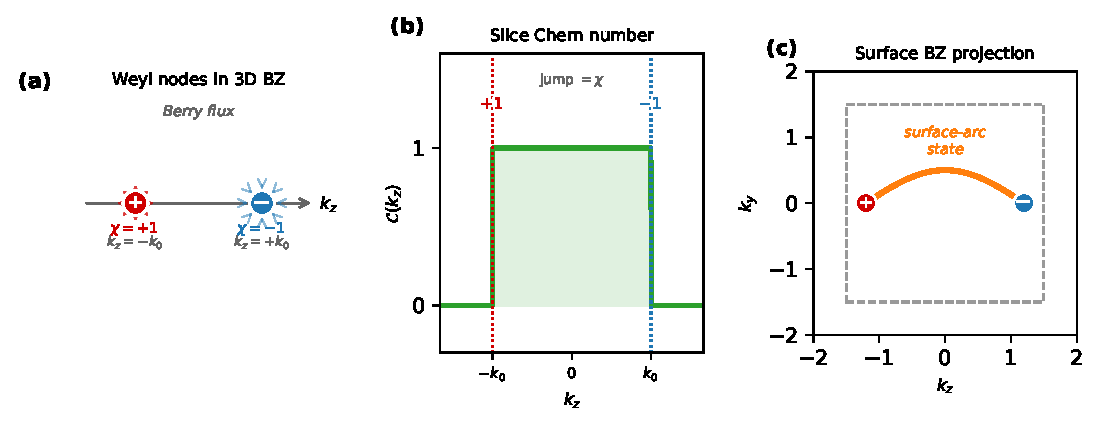
\includegraphics[width=0.95\textwidth]{figures/fig_ch15_weyl_chern_slices_step236.pdf}
  \caption{Weyl points as Berry-curvature monopoles.
  \textbf{(a)}~Two Weyl nodes at $k_z=\pm k_0$ with chiralities
  $\chi=+1$ (source, red) and $\chi=-1$ (sink, blue); Berry-flux
  arrows indicate the monopole and anti-monopole character.
  \textbf{(b)}~The 2D slice Chern number $\Chern(k_z)$ jumps by
  $+\chi$ when the slice passes through a Weyl node, giving the
  step function $0\to 1\to 0$ for the lower band.
  \textbf{(c)}~Surface Brillouin zone showing the photonic
  surface-arc state (orange) connecting the projected Weyl nodes.
  The arc exists only for $k_z$ values where $\Chern(k_z)\neq 0$,
  as required by the bulk--edge correspondence applied slice by
  slice.}
  \label{fig:ch15-weyl-chern-slices}
\end{figure}

\subsection{Fermi-arc connectivity}
\label{sec:ch15-connectivity}

The connectivity of Fermi arcs is topologically constrained: each Weyl
point must be the endpoint of exactly $|\chi|$ arcs.  For charge-1
Weyl points ($|\chi|=1$), each is connected to exactly one other Weyl
point of opposite chirality by a single arc.  The arc cannot terminate
in the interior of the surface Brillouin zone.

When multiple pairs of Weyl points are present, the arcs can connect
them in different patterns, depending on the surface orientation and
termination.  Different surface terminations of the same bulk crystal
can produce different arc connectivity patterns.

\section{Experimental observation of photonic Weyl points}
\label{sec:ch15-experiments}

\subsection{Microwave experiments}
\label{sec:ch15-microwave}

The first experimental observations of photonic Weyl points were achieved
in 3D-printed metallic structures at microwave frequencies
\cite{noh2017experimental,price2022roadmap}.  The
experiments measured:
\begin{itemize}
  \item The bulk band structure, confirming the linear dispersion near
  the Weyl point.
  \item The surface states, showing the characteristic Fermi-arc
  connectivity.
  \item The robustness of the Weyl points to perturbations (they move
  but do not gap).
\end{itemize}

\subsection{Photonic crystal observations}
\label{sec:ch15-photonic-obs}

Weyl points have also been observed in
\cite{ozawa2018topological,noh2017experimental}:
\begin{itemize}
  \item Stacked dielectric photonic crystal slabs with controlled
  interlayer coupling.
  \item Chiral woodpile structures (alternating layers of rods with
  rotation between layers).
  \item Metamaterial waveguide arrays.
\end{itemize}

\section{Nodal lines and higher-order degeneracies}
\label{sec:ch15-nodal}

\subsection{Nodal lines}
\label{sec:ch15-nodal-lines}

A \emph{nodal line} is a closed loop of band degeneracies in
$\kvec$-space.  Unlike Weyl points (which are 0-dimensional), nodal
lines are 1-dimensional objects.  They carry a Berry phase of $\pi$
along any path linking the loop:
\begin{equation}\label{eq:ch15-nodal-berry}
  \gamma = \oint_C\Aberryvec\cdot\dd\kvec = \pi
  \quad\text{for } C \text{ linking the nodal line once.}
\end{equation}
This $\pi$ Berry phase is protected by a mirror or glide symmetry that
forces the eigenstates on the nodal line to be degenerate.

Nodal-line photonic crystals produce ``drumhead'' surface states:
surface states that fill a 2D region in the surface Brillouin zone
bounded by the projection of the nodal line, rather than forming a 1D
arc.

\subsection{Multi-Weyl points}
\label{sec:ch15-multi-weyl}

At high-symmetry points in crystals with $C_n$ ($n\geq 3$) rotational
symmetry, Weyl points can carry higher topological charges $|\chi|>1$.
A \emph{double-Weyl point} ($|\chi|=2$) has quadratic dispersion in
the plane perpendicular to the rotation axis and linear dispersion
along it:
\begin{equation}\label{eq:ch15-double-weyl}
  H = v_\perp(k_+^2\sigma_+ + k_-^2\sigma_-) + v_z\delta k_z\sigma_z\,,
\end{equation}
where $k_\pm=\delta k_x\pm\ii\delta k_y$ and
$\sigma_\pm=(\sigma_x\pm\ii\sigma_y)/2$.

A double-Weyl point sources two units of Berry flux and is the endpoint
of two Fermi arcs.

\subsection{Dirac points in 3D}
\label{sec:ch15-3d-dirac}

When both $\Top$ and $\Pop$ are present, the minimal degeneracy at a
band crossing is a four-fold \emph{Dirac point}: two overlapping Weyl
points of opposite chirality.  Breaking $\Top$ or $\Pop$ splits the
Dirac point into a pair of Weyl points.  The separation between the
Weyl points is controlled by the symmetry-breaking strength.

\section{Connection to Maxwell equations}
\label{sec:ch15-maxwell}

The Weyl-point physics described in this chapter is derived from the
same Maxwell eigenvalue problem $\Maxop(\kvec)\mathbf{u}=\omega\Mmat
\mathbf{u}$ that underlies the entire book.  The 3D extension is
straightforward: $\kvec$ now has three components, the Brillouin zone
is a 3D torus $T^3$, and the Berry curvature is a vector field in
3D $\kvec$-space.

The electromagnetic inner product
$\langle\mathbf{u}|\Mgmat|\mathbf{u}'\rangle$ remains essential for
the correct definition of Berry curvature and topological charges.
Using the wrong inner product would give incorrect monopole charges
and Fermi-arc predictions.

The slice Chern number $\Chern_n(k_z)$ is computed using the same
plaquette formula of \chref{ch:computing-chern}, applied to the
2D slice at fixed $k_z$.  The Wilson-loop method extends naturally:
the Wilson loop at each $(k_y,k_z)$ gives a Zak phase whose winding
in $k_y$ at fixed $k_z$ yields $\Chern_n(k_z)$.

\section{Three-dimensional gapped topological phases}
\label{sec:ch15-3d-gapped}

While Weyl semimetals are gapless---their defining feature is the
point-like band touching---three-dimensional photonic systems can also
host \emph{gapped} topological phases
\cite{yang2026non,armitage2017weyl}.  These are the 3D analogs of
the 2D Chern insulator and the 2D $\mathbb{Z}_2$ topological
insulator: the bulk has a complete frequency gap, and the topology
manifests as robust surface states on every boundary.

\subsection{From 2D to 3D: stacking and strong invariants}
\label{sec:ch15-stacking-gapped}

A simple route to a 3D topological insulator begins with a stack of 2D
topological layers.  If each layer is a 2D Chern insulator with
$\Chern=1$, the stacked system has chiral surface states on every face
perpendicular to the stacking axis.  This ``weak'' topological
insulator inherits its topology from the 2D layers and is vulnerable to
disorder that mixes layers.

A \emph{strong} 3D topological insulator, by contrast, has surface
states on \emph{every} surface orientation, protected by a truly 3D
topological invariant.  In electronic systems, this invariant is the
$\mathbb{Z}_2$ index protected by time-reversal symmetry
(Kane and Mele, 2005; Fu, Kane, and Mele, 2007).  The photonic analog
requires a pseudo-time-reversal symmetry, typically constructed from
bianisotropic coupling between TE-like and TM-like modes.

\subsection{The bianisotropic route to a 3D photonic TI}
\label{sec:ch15-bianisotropic-3d}

The most successful experimental realisation of a 3D photonic
topological insulator was demonstrated by Yang et~al.\
\cite{yang2018realization} using an array of metallic split-ring
resonators (SRRs) embedded in a dielectric host.  The SRRs provide
strong bianisotropic coupling---the magneto-electric cross-terms
$\xit$ and $\zetat$ of the material matrix
(Appendix~\ref{app:material-tensors})---which plays the role of
spin-orbit coupling in the electromagnetic context.

The key design principle is as follows.  Each SRR supports both an
electric resonance (responding to $\Efield$) and a magnetic resonance
(responding to $\Hfield$) at the same frequency, with a cross-coupling
$\xit\neq 0$ that mixes the two.  When the SRRs are arranged on a
3D lattice, the resulting photonic band structure exhibits a complete
bulk bandgap with topologically nontrivial bands below the gap.

The measured bulk bandgap extended from approximately $4.3$ to
$6.0\;\mathrm{GHz}$ (a relative bandwidth exceeding $25\%$), which is
remarkably large compared to earlier 2D photonic topological gaps of a
few percent \cite{ozawa2018topological}.  The large gap makes the
surface states well-resolved and experimentally accessible.

\subsection{Surface Dirac cones}
\label{sec:ch15-surface-dirac}

The hallmark of a 3D gapped topological insulator is a single
\emph{Dirac cone} on each surface---a linearly dispersing surface
state that is topologically protected against backscattering by
disorder or defects.

In the Yang et~al.\ experiment, near-field scanning measurements of
the surface electromagnetic field revealed:
\begin{enumerate}
  \item A surface state with linear (conical) dispersion centred at
  $5.1\;\mathrm{GHz}$, lying within the bulk bandgap.
  \item Robust surface propagation along non-planar surfaces,
  including bends and corners, without backscattering.
  \item A penetration depth of approximately $10\;\mathrm{mm}$ into
  the bulk, consistent with the exponential localisation expected from
  a gapped topological surface state.
\end{enumerate}

The surface Dirac cone should be contrasted with the Fermi arcs of a
Weyl semimetal (\secref{sec:ch15-surface}).  A Fermi arc is an
\emph{open} curve in the surface Brillouin zone, terminating at
projected Weyl points; a surface Dirac cone is a \emph{closed} conical
dispersion centred at a time-reversal-invariant momentum.  The arc
exists because the bulk is gapless (Weyl points); the Dirac cone exists
because the bulk is fully gapped.

\subsection{Comparison of 3D gapped and gapless phases}
\label{sec:ch15-gapped-vs-gapless}

The following table summarises the key differences between 3D gapless
(Weyl) and gapped (topological insulator) phases in photonic crystals.

\begin{center}
\begin{tabular}{lcc}
  \toprule
  & \textbf{3D Weyl semimetal} & \textbf{3D topological insulator} \\
  \midrule
  Bulk gap & none (point nodes) & complete frequency gap \\
  Topological invariant & monopole charge $\chi$ & $\mathbb{Z}_2$ or
    3D Chern numbers \\
  Surface states & open Fermi arcs & closed Dirac cone \\
  Symmetry requirement & break $\Top$ or $\Pop$ & pseudo-$\Top$ from
    bianisotropy \\
  Robustness & nodes move, do not gap & gap persists under all
    symmetry-preserving perturbations \\
  Key photonic experiment & Noh et~al.\ (2017) & Yang et~al.\ (2019) \\
  \bottomrule
\end{tabular}
\end{center}

Both phases are derived from the same 3D Maxwell eigenproblem
$\Maxop(\kvec)\mathbf{u}=\omega\Mmat\mathbf{u}$, but with different
material symmetries: broken $\Pop$ or $\Top$ for Weyl semimetals,
and engineered pseudo-$\Top$ for gapped topological insulators.

\subsection{Towards optical-frequency 3D topological insulators}
\label{sec:ch15-optical-3dti}

The Yang et~al.\ demonstration operated at microwave frequencies, where
SRR fabrication is straightforward.  Extending 3D photonic topological
insulators to optical frequencies is an active research frontier
\cite{price2022roadmap}.  The challenges include fabricating 3D
nanostructures with precise bianisotropic response and maintaining a
sufficiently large bandgap relative to fabrication imperfections.  Recent
proposals based on all-dielectric metacrystals and chiral woodpile
structures suggest that optical-frequency 3D topological gaps may be
achievable with current nanofabrication technology \cite{khanikaev2016three}.

\section{Type-I and type-II Weyl points}
\label{sec:ch15-types}

Weyl points come in two types, distinguished by their isofrequency
surfaces \cite{chen2021ideal}.  A type-I Weyl point has a point-like Fermi surface at the
Weyl frequency: the isofrequency contour shrinks to a single point,
with the dispersion forming an upright cone
$\omega=\omega_W\pm v|\delta\kvec|$.

A type-II Weyl point has a tilted cone, so that the isofrequency
surface at $\omega=\omega_W$ is not a point but a pair of electron-
and hole-like pockets touching at the Weyl point.  The effective
Hamiltonian is
$H=v_t k_z\sigma_0 + v(k_x\sigma_x+k_y\sigma_y+k_z\sigma_z)$,
where $v_t>v$ is the tilt velocity.  The tilt breaks Lorentz
invariance but does not change the topological charge of the Weyl
point \cite{noh2017experimental,ozawa2018topological}.

Type-II Weyl points were first observed in photonics by Noh et~al.\
(2017) using a laser-written waveguide array.  The waveguides were
arranged in a face-centred geometry with controlled interlayer
coupling, producing tilted Weyl cones in the propagation-constant
spectrum.  The type-II nature was confirmed by observing the
characteristic ``bowtie'' isofrequency contour using Fourier-space
imaging \cite{noh2017experimental}.

\section{Nodal lines and drumhead surface states}
\label{sec:ch15-nodal-lines-drumhead}

When two bands cross along a line in the 3D Brillouin zone rather
than at an isolated point, the crossing is called a \emph{nodal line}.
Nodal lines can be stabilised by crystal symmetries (e.g.\ mirror or
glide symmetries) and carry a $\pi$ Berry phase around any loop
encircling the line, analogous to the $\pi$ Berry phase at a 2D Dirac
point \cite{kim2015dirac,ozawa2018topological}.

The bulk-boundary correspondence for nodal lines predicts
\emph{drumhead surface states}: flat or nearly flat bands that fill
the interior of the projected nodal line on the surface Brillouin
zone.  These states have a high density of states and are of interest
for enhanced light--matter interaction.

Nodal-line photonic crystals have been realised using dielectric
structures with carefully designed symmetries.  The drumhead states
have been observed as bright, nearly dispersionless features in
angle-resolved transmission measurements
\cite{price2022roadmap}.

\section{Experimental platforms for 3D photonic topology}
\label{sec:ch15-3d-platforms}

Three-dimensional photonic topological phases have been demonstrated
on several platforms:

Laser-written waveguide arrays in fused silica provide type-II Weyl
points and Fermi-arc surface states at optical wavelengths
($\lambda=633\;\mathrm{nm}$).  The paraxial propagation approximation
maps the 3D waveguide structure onto a (2+1)D tight-binding model
with the propagation direction playing the role of time
\cite{noh2017experimental,rechtsman2013photonica}.

Metallic photonic crystals with gyroid or diamond symmetry can
support complete 3D band gaps with nontrivial topology.  The
Weyl points appear as pairs of opposite-charge monopoles in the
3D Brillouin zone, connected by surface Fermi arcs on any
termination \cite{ozawa2018topological}.

Bianisotropic metamaterials (split-ring resonator arrays) realise
3D topological insulators with surface Dirac cones, as discussed in
Chapter~\ref{ch:microwave-crystal}
\cite{yang2018realization,price2022roadmap}.

\section{Surface Dirac cones and topological surface states}
\label{sec:ch15-surface-dirac-cone}

A 3D photonic topological insulator---a material with a nontrivial
$\mathbb{Z}_2$ invariant---supports gapless surface states that form
a Dirac cone in the surface Brillouin zone.  These surface Dirac
cones are the 3D analog of the chiral edge modes of a 2D Chern
insulator: they are topologically protected and cannot be gapped by
any surface perturbation that preserves time-reversal symmetry.

The surface Dirac cone was first observed experimentally by Yang
et~al.\ (2019) in a bianisotropic metamaterial of double split-ring
resonators arranged in a body-centred cubic lattice.  Angle-resolved
transmission measurements on a cleaved crystal surface revealed a
linear dispersion cone at $\bar{\Gamma}$ in the surface Brillouin zone,
with the Dirac frequency at $5.1\;\mathrm{GHz}$ inside the bulk gap
from 4.3 to $6.0\;\mathrm{GHz}$
\cite{yang2018realization,ozawa2018topological}.

The robustness of the surface Dirac cone was confirmed by introducing
surface disorder (randomly removing $10\%$ of the surface resonators)
and observing that the Dirac cone remained intact, with only a slight
broadening of the surface states.  This is consistent with the
$\mathbb{Z}_2$ protection: the surface Dirac cone can be shifted in
energy or broadened by disorder, but it cannot be gapped
\cite{price2022roadmap}.

\subsection{Comparison table: 2D edge modes versus 3D surface states}
\label{sec:ch15-comparison-2d-3d}

The 2D and 3D cases share the same topological origin but differ in
dimensionality and symmetry:
\begin{center}
\begin{tabular}{lll}
  \toprule
  Property & 2D Chern insulator & 3D topological insulator \\
  \midrule
  Bulk invariant & Chern number $\Chern\in\mathbb{Z}$ &
    $\mathbb{Z}_2$ index $\nu\in\{0,1\}$ \\
  Boundary states & chiral edge modes & surface Dirac cone \\
  Protection & against all gap-preserving & against $\Top$-preserving \\
  & perturbations & perturbations \\
  Requires $\Top$ breaking & yes & no \\
  Min.\ boundary modes & $|\Chern|$ & 1 Dirac cone \\
  \bottomrule
\end{tabular}
\end{center}

\section{Photonic Weyl semimetal experiments}
\label{sec:ch15-weyl-experiments}

The theoretical prediction of Weyl points in photonic crystals was
confirmed experimentally in several landmark experiments that
directly observed the key signatures: bulk conical dispersions,
surface Fermi arcs, and robustness against perturbations.

\subsection{The double-gyroid photonic crystal}
\label{sec:ch15-double-gyroid}

The first experimental observation of photonic Weyl points was
reported by Lu et~al.\ (2015) in a double-gyroid photonic crystal
at microwave frequencies \cite{price2022roadmap}.  The double
gyroid is a bicontinuous structure with body-centred cubic symmetry
described by the level-set equation
\begin{equation}\label{eq:ch15-gyroid-level-set}
  f(\rvec) = \sin(2\pi x/a)\cos(2\pi y/a)
  + \sin(2\pi y/a)\cos(2\pi z/a)
  + \sin(2\pi z/a)\cos(2\pi x/a)\,,
\end{equation}
where the two gyroid networks occupy the regions $f>t_0$ and
$f<-t_0$ for a threshold $t_0$.  The structure was fabricated by
3D-printing metallic scaffolds with lattice constant $a=13\;\mathrm{mm}$,
operating in the 5--8~GHz range.

By breaking either time-reversal or inversion symmetry (achieved by
coating one of the two gyroid networks with a metallic layer to
destroy inversion), the authors lifted a four-fold line degeneracy
into pairs of Weyl points with opposite chirality.  Angle-resolved
microwave transmission measurements mapped the bulk band structure
and confirmed the linear conical dispersion near the Weyl frequencies
\cite{ozawa2018topological}.

\subsection{Surface Fermi arcs}
\label{sec:ch15-fermi-arcs-exp}

The surface Fermi arc is the defining experimental signature of a
Weyl semimetal: it is an open contour of constant-frequency surface
states that connects the projections of two Weyl points of opposite
chirality onto the surface Brillouin zone.

The existence of Fermi arcs follows from a topological argument.
Consider a closed loop $\mathcal{C}$ in the surface Brillouin zone
that encircles the projection of a single Weyl point.  The Chern
number of the occupied bands evaluated on $\mathcal{C}$ is
$\Chern(\mathcal{C})=\pm 1$, implying that at least one surface
band must cross the Weyl-point frequency within $\mathcal{C}$.
Since the surface band cannot form a closed contour (it would then
encircle equal numbers of positive and negative chirality
projections and carry zero Chern flux), it must terminate at the
Weyl-point projections.  The resulting open arc is the Fermi arc.

In the double-gyroid experiment, surface Fermi arcs were observed by
measuring the near-field intensity distribution on a cleaved crystal
surface.  The arc-like surface dispersion was clearly visible in the
angle-resolved transmission, connecting pairs of projected Weyl
points as predicted by the bulk-boundary correspondence
\cite{ozawa2018topological,price2022roadmap}.

\subsection{Type-II Weyl points in photonic systems}
\label{sec:ch15-type-ii-exp}

Type-II Weyl points, introduced in \secref{sec:ch15-types}, are
characterised by a strongly tilted cone that intersects the
constant-frequency surface to form electron and hole pockets.  In a
photonic crystal, the ``pockets'' are regions of propagating bulk
modes that coexist with the Weyl frequency, leading to qualitatively
different surface-state physics: the Fermi arcs connect not only the
Weyl-point projections but also merge with the bulk pocket
projections \cite{ozawa2018topological}.

Noh et~al.\ (2017) reported the first observation of type-II Weyl
points in a photonic system using a stacked bilayer photonic crystal
\cite{noh2017experimental}.  The structure consisted of alternating
layers of hexagonal photonic crystal slabs with different in-plane
geometries, creating a three-dimensional photonic crystal with
broken inversion symmetry.  The strongly tilted conical dispersion
was confirmed by angle-resolved reflection measurements, and the
characteristic electron--hole pocket structure was observed at
frequencies near the Weyl point.

\subsection{Ideal Weyl points and minimal photonic designs}
\label{sec:ch15-ideal-weyl}

An ``ideal'' Weyl semimetal has its Weyl points located exactly at the
Fermi level (or, in the photonic case, at a frequency isolated from
all other bands), so that the only states at that frequency are the
Weyl cones and the surface arcs.  This ideal condition maximises the
length of the Fermi arcs and the surface-state density of states.

Yang et~al.\ (2018) realised an ideal Weyl system using a
saddle-shaped metallic inclusion in a body-centred cubic unit cell
\cite{yang2018realization,yang2017discovery}.  The design produced Weyl points that
were separated from all other bands by a complete frequency gap,
giving the longest possible Fermi arcs spanning the entire surface
Brillouin zone.  The experiment was performed at microwave
frequencies with 3D-printed metallic structures, and the surface arcs
were mapped by near-field scanning measurements.

\begin{figure}[t]
  \centering
  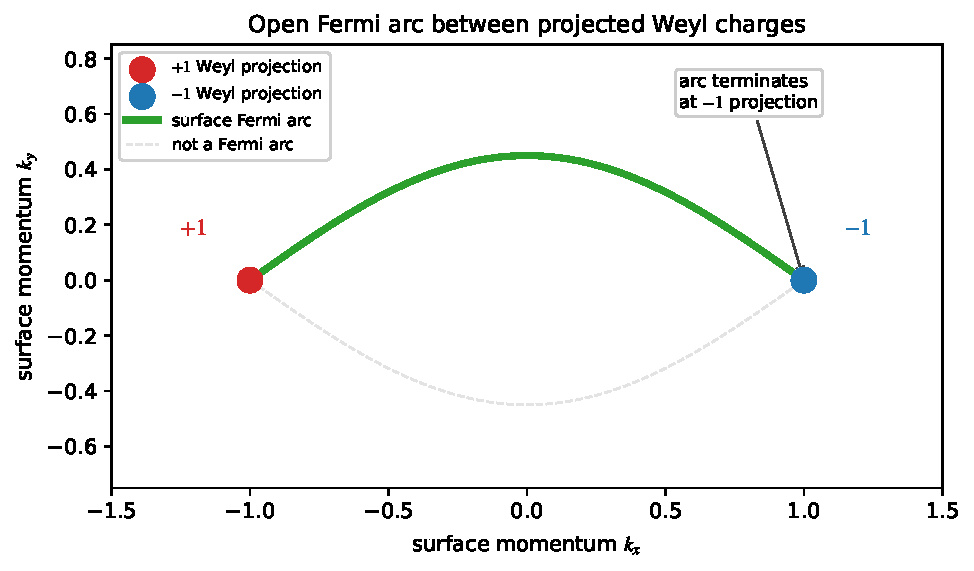
\includegraphics[width=0.78\textwidth]{figures/fig_ch15_weyl_fermi_arc.pdf}
  \caption{A surface Fermi arc connects projected Weyl charges of opposite
  chirality.  Unlike an ordinary constant-frequency contour, the arc is open:
  it terminates on the surface projections of bulk Weyl points, expressing
  the Chern-number jump across the Weyl node.}
  \label{fig:ch15-weyl-fermi-arc}
\end{figure}

\section*{Exercises}

\begin{exercise}
  Compute the Berry curvature of the lower band of the isotropic Weyl
  Hamiltonian $H=v(\delta k_x\sigma_x+\delta k_y\sigma_y
  +\delta k_z\sigma_z)$ and verify that it has the monopole form
  \eqref{eq:ch15-general-berry} with $\chi=+1$.
\end{exercise}

\begin{exercise}
  Show that no $2\times 2$ Hermitian perturbation can gap the 3D Weyl
  Hamiltonian \eqref{eq:ch15-weyl-hamiltonian}.  \emph{Hint:} write the
  most general $2\times 2$ Hermitian matrix $\delta H=\sum_a\delta d_a
  \sigma_a+\delta d_0\mathbf{I}$ and show that adding it to $H_W$ only
  shifts the Weyl point.
\end{exercise}

\begin{exercise}
  For a pair of Weyl points at $\kvec_\pm=(0,0,\pm k_0)$ with
  chiralities $\chi_\pm=\pm 1$, compute the slice Chern number
  $\Chern(k_z)$ for $|k_z|<k_0$, $|k_z|>k_0$, and $k_z=\pm k_0$.
  Use this to derive the existence and extent of the Fermi arc on the
  $(001)$ surface.
\end{exercise}

\begin{exercise}
  Explain why Weyl points require the breaking of either $\Top$ or
  $\Pop$ (or both).  \emph{Hint:} show that $\Top\Pop$ symmetry forces
  the eigenstates to be at least doubly degenerate at every $\kvec$ in
  a system where both are preserved.
\end{exercise}

\begin{exercise}
  A photonic nodal line in a 3D crystal is a closed loop in
  $\kvec$-space where two bands are degenerate.  Show that the Berry
  phase $\gamma=\oint_C\Aberryvec\cdot\dd\kvec$ for a path $C$ linking
  the nodal line once is quantised to $\pi$.  What symmetry protects
  this quantisation?
\end{exercise}

\begin{exercise}
  For a double-Weyl point with Hamiltonian \eqref{eq:ch15-double-weyl},
  compute the Berry flux through a sphere enclosing the degeneracy and
  verify that the topological charge is $|\chi|=2$.
\end{exercise}

\begin{exercise}
  Consider a 3D photonic crystal with a single pair of Weyl points on
  the $k_z$ axis.  If the crystal is truncated to form a slab of
  thickness $L$ in the $x$-direction, describe qualitatively how the
  Fermi arcs on the top and bottom surfaces connect through the slab
  as $L$ decreases.
\end{exercise}
